\documentclass{lsstbeamer}

\title[LSST Docs]{ LSST Documentation  }

\author[W. O'Mullane ]{William O'Mullane }

\date[ 11/01/2017]{Jan  11$^{th}$ 2017 DMLT Tucson}

\institute[LSST Corporation]{LSST\\Tucson\\Arizona}
\begin{document}

% ----------------------



\frame {
  \frametitle{  Flight Operations Procedures in MOC}
\vspace{-0.4cm}
\begin{center}
   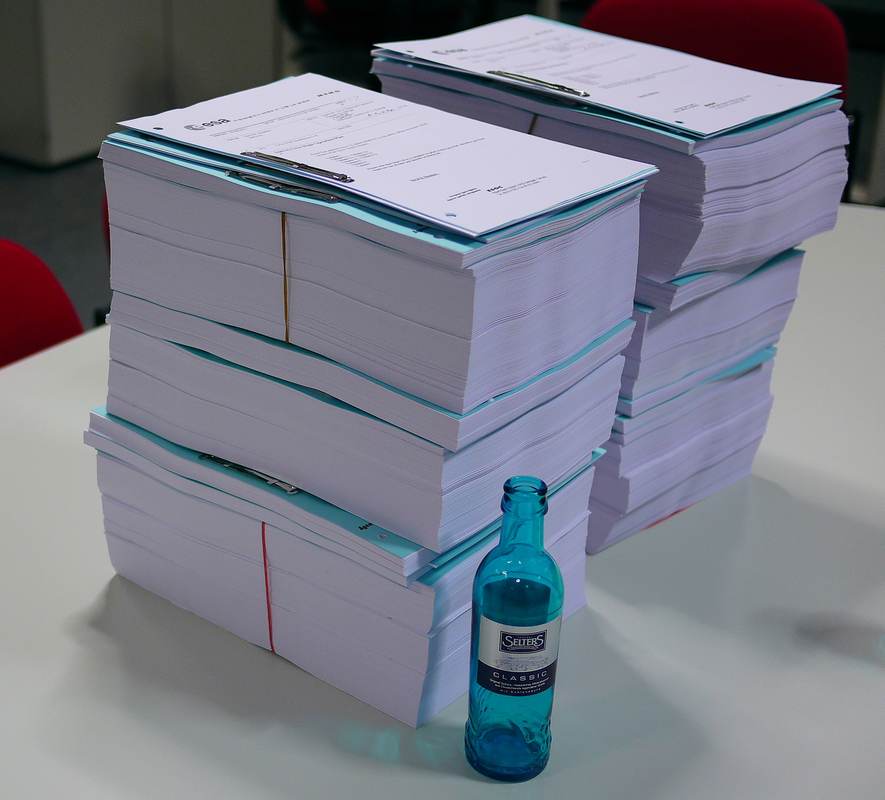
\includegraphics[width=0.6\textwidth,trim=0cm 0cm 0cm 0cm]{images/fops}\\
\end{center}
\vspace{-7pt}
The FOP is followed by the spacecraft operators - the paper copy is just in case the computers fail - could be useful!
\begin{center}
\vspace{-5pt}
{\color{red} But we should avoid {\em write only} documents.}
\end{center}
}




\frame[allowframebreaks]  {\frametitle{  Impression LSST  DM docs }

\begin{itemize}
  \item  No standard - no Overview  of DM docs I could find -   some web pages 
   
\begin{itemize}
   \item did not find a document management plan for DM ..
  \item LDM-493 .. covers some aspects .. but still no Doctree - templates ?
  \item not nice to have tex/markdown/word others ?   Markdown ok for implementation docs but for technotes for science notes?
  \item Hence no clear project {\em identity} - DM team DOCS should scream \\ {\color{blue} \Large \em DM TEAM} consistently 
\end{itemize}
  \item Mention made of LPM-051 .. but is DM following this ? Or just not declaring controlled documents .. {\em prefer term ISSUED} rather than controlled
        \begin{itemize}

   \item docushare  is the LSST repo but DM docs seem old (did find some from KT) - should all issued docs be there (I think so ..)
        \item would expect to find all Technotes from DM in docushare .. like in a technotes folder ... SQR-006 gives an API which I may be able to use - should not be this hard.
        \end{itemize}
\item would like to find all draft docs in one DM repo ..
    \item everything is {\em referenceable} - but I do not find a single bibtex database or such for issued docs ..  (Gaia livelink metadata is exported as a bibtex every night)


\item {\color{red} All products should be listed and for each product the set of docs expected and the dates}  
        \begin{itemize}
	\item each document type is  targeted at a different audience (e.g. Requirement, Design/Implementation, Installation, User \ldots 
	\item not all products have all document types). 
        \end{itemize}
  \item  LDTN-030 - ok for code documentation -  understand its evolving-
        \begin{itemize}
        \item overlaps LDM-493 somewhat - Why so many documentation projects - should we have ONE for DM ?
        \item Provides document shards - no structure - how do you get a an old version (users will not get from git) .. LTD perhaps - but not well explained.
	\item Audience seems too broad to cover with one type of document
        \item This "In our case, the situation is complicated by the fact that Data Management software is being built by multiple teams across many coupled repositories. Taken together, the software repositories of the Data Management System are typically called the Stack, but not all parts of the Stack are used together. There are server-side database and display components, as well as pipelines algorithms bound together with middle ware." {\color{red} does not sound like good system engineering is in place .. }
        \item Unclear in a massive web how one  can check consistency to any given level for docs .. {\color{red} Potential  problem for reviewers}
        \end{itemize}
\end{itemize}
 
}

% ----------------------
\end{document}
